\chapter{The Lattice Boltzmann Algorithm}
\section{General Description}
Now that we have overviewed the pertinent concepts, we can proceed to the particulars of this implementation.

As previously asserted, the heart of the Lattice-Boltzmann Algorithm lies on its discretization of the phase space\cite{franco} \cite{integerLatticeDynamics}.\\

To discretize the phase space, one must first choose the region to simulate. In this work, we name the extremal values in the $w$ axis of the phase space $W_{min}$ and $W_{max}$.
Then, one has to fix either the size of the grid or the size of the lattice.
We name the length of the grid in the $w$ axis $N_w$ (i.e. $N_x$ or $N_{vz}$).
The size of the lattice in the $w$ axis (which we are going to name $dw$) and the extremal values are related by:\\

\begin{equation}
dw = \frac{W_{max}-W_{min} }{N_w} 
\end{equation}\\

In this work we are going to use the phase-space mass density, which means that $\f \dd \vb{r} \dd \vb{v}$ is the density of dark matter whose position is between $\vb{r}$ and $\vb{r} + \dd \vb{r}$, and its velocity is between $\vb{v}$ and $\vb{v} + \dd \vb{v}$.
Now that we have properly defined the phase space grid, we can proceed to initialization.
For simplicity, we choose gaussian initial conditions given by:


\begin{equation}
\f[0]= A \exp{-\frac{\vb{r}^2}{\sigma_r^2} - \frac{\vb{v}^2}{\sigma_v^2}}
\end{equation}


Where $\f[0]$ is the initialization of the phase space density, $A$ is an indirect measure of the total mass in the system, $\vb{r}$ is the vector $(x,y,z)$, $\vb{v}$ is the vector $(vx,vy,vz)$, and $\sigma_i$ are a measure of the width of the gaussian profile in the given axis. Note that we use a single width for the spatial axis and a single width for the velocity axis.\\


After initialization, the system evolves by the action of the Louville operator and the Collisional operator. The schematics of the algorithm can be seen easily in figure  \ref{flowchart}.

\begin{figure}[H]
    \centering
    %\includegraphics[width=10cm,height =7cm]{Diapositiva1.jpg}
    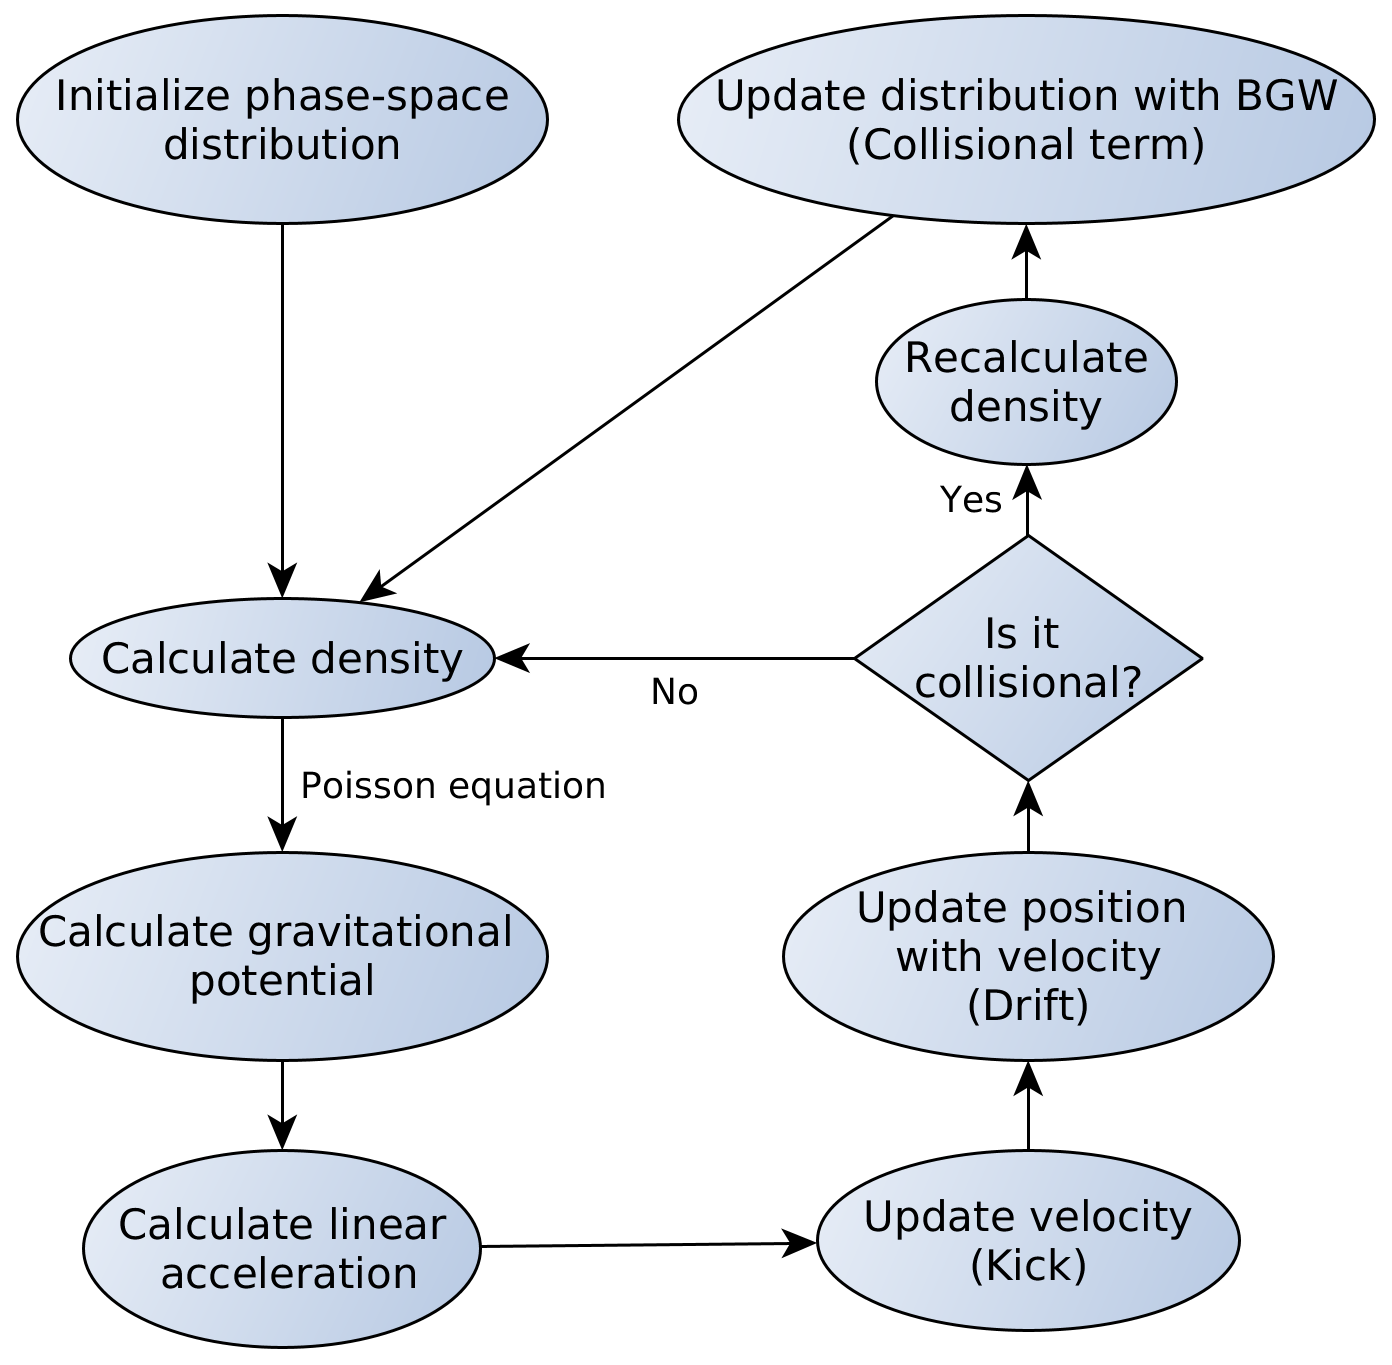
\includegraphics[scale=0.2]{imag/flowchart.png}
    \caption{Flowchat of the algorithm.}
    \label{flowchart}
\end{figure}

Now that we have defined the phase-space, we can obtain the spatial density of matter by integrating the phase space:
 
\begin{equation}
\label{defDens0}
\dens[t] = \int_{-\infty}^{\infty} \! \f[t] \, \dd \vb{v}.
\end{equation}

When evaluating in the lattice the integral becomes a sum over the entire velocity lattice:

\begin{equation}
\label{defDens}
\dens[t] = \sum_{\vb{V}_{min}}^{\vb{V}_{max}} \f[t] \, \dd \vb{v}
\end{equation}

and during initialization:

\begin{equation}
\dens[0] = \sum_{\vb{V}_{min}}^{\vb{V}_{max}} \f[0] \, \dd \vb{v}
\end{equation}

Once we have calculated the density, we solve the Poisson equation to obtain the potential due to gravitational interaction:	\cite{integerLatticeDynamics}\\

\begin{myequation}
\laplacian \pot = 4 \pi G \dens
\end{myequation}\\
%TODO:añadir \\
Where $\pot$ is the gravitational potential and $G$ is the gravitational constant.
To solve the Poisson equation we use the Fourier pseudo-spectral method, which allows for very fast numerical solutions by making use of the Fast Fourier Transform algorithm. The idea is simply to apply a Fast Fourier Transform (FFT) to the density, then solve the equation in the Fourier space, and then apply an inverse transform (IFFT). In the Fourier space the Poisson equation is given by\cite{freePoisson} \cite{computerUsingParticles}\\

\begin{myequation}
\lambda_{\vb{k}}^2 \hat{\Phi}(\vb{k},t) = 4 \pi G \hat{\rho}(\vb{k},t)
\end{myequation}\

%\vspace{1mm}

Where $\hat{g}(\vb{k},t)$ is the Fourier transform of $g(\vb{r},t)$, and $\lambda_{\vb{k}}$ is a constant that depends on the size of the lattice and the wavevector $\vb{k}$.
$\lambda_{\vb{k}}$ is calculated according to the approximation scheme used to solve the equation.
In the the pseudo-spectral approximation, $\lambda_{\vb{k}}$ is given by:\\

\begin{myequation}
\lambda_{\vb{k}}^2 = \qty(\frac{2 \pi k_x}{X_{max} - X_{min}})^2 + \qty(\frac{2 \pi k_y}{Y_{max} - Y_{min}})^2 + \qty(\frac{2 \pi k_z}{Z_{max} - Z_{min}})^2
\end{myequation}\\

Therefore, solving the Poisson equation in the Fourier space is reduced to simple arithmetic.
Thanks to the highly efficient implementations of the Fast Fourier Transform Algorithm available nowadays, solving the Poisson equation takes very little time and computational resources.
In this work we use the Fastest Fourier Transform of the West\cite{FFTW} subroutine to handle the Fast Fourier Transforms.\\
%TODO: incluir cita a FFTW

Once we have calculated potential, obtaining the acceleration is straight-forward:\\

\begin{myequation}
\acce = -\grad \pot
\end{myequation}\\

Which, in the context of the lattice can be calculated simply with a central difference numerical derivative.\\


Now, in order to update the phase space, we must first define the time interval to simulate: we name $N_t$ the number of time intervals to simulate and $\dd t$ the length of each of such intervals.
After calculating the acceleration and defining $\dd t$, we can update our phase space, the subtlety here is that we will only use integer arithmetic, which means that we do not exactly care for the change in velocity during a time $\dd t$ but for how many cells in the phase space that change represents. This is modeled by:

\begin{myequation}
\vb{v}_{n+1} = \vb{v}_n + \toInt{\vb{a}_n \dd t}
\end{myequation}

With $\toInt{x}$ representing the operator \tqt{to nearest integer}, so that $\vb{v}$ and $\toInt{\vb{a} \dd t}$ are vectors of integers and $n$ represents the time instant. The update of the velocity is known as \tqt{kick}. Analogously, the update of the position is known as \tqt{drift}, and is given by:

\begin{myequation}
\vb{r}_{n+1} = \vb{r}_n + \toInt{\vb{v}_n \dd t}
\end{myequation}

Using only integer arithmetics allows for the elimination of the rounding error but introduces lattice noise. Regardless, this method creates a one to one map with the continous solution.\cite{franco} \cite{integerLatticeDynamics}\\

The \tqt{kick} and \tqt{drift} together are known as the \tqt{Streaming} step, and it represents the classical movement of particles under a potential but without considering the collision of particles. If we want a collisionless simulation, we can just calculate again the density and continue the algorithm from there. If we want a collisional simulation, we must define a collisional step.\\

\section{The Collisional Step}
As previously mentioned, solving the collisional integral $C[f]$ is not straight-forward, as it depends on the modeling of the short range interactions that we decide to assign to the dark matter particle. Given that the short range interaction of dark matter is unknown, we avoid using an specific description of the microscopic interactions and choose to use a mesoscopic approach, as discussed in section \ref{bgk}. The BGK collisional operator is given by:\\

\begin{equation}
C[f] = -\frac{1}{\tau}(\f - f_e(\rv))
\end{equation}\\

Which in the context of the direct integration scheme used in the simulation becomes:

\begin{myequation}
f(\vb{r} + \vb{v} \dd t,\vb{v},t) = \f - \frac{\dd t}{\tau}(\f - f_e(\rv))
\end{myequation}

The idea behind this approach is to recover the macroscopic description of the fluid without committing to a particular microscopic description. In this scenario, the macroscopic effects of the collisions is a local relaxation towards equilibrium, which the BKG operator models using a relaxation time $\tau$ and a local equilibrium distribution $f_e(\rv)$. \\


In order to implement a collisional operator we add a collisional step after the streaming step, in which the system performs a relaxation with characteristic (relaxation) time $\tau$ towards the local equilibrium distribution $f_e(\rv)$. 
It is important to notice that the BGK collisional operator is a \emph{scattering} operator and does not includes annihilation or creation of particles. \\

After defining the collisional term, we have to choose a distribution fuction $f_e(\rv)$. We claim that the phase space distribution relaxes towards equilibrum, which means a displacement in the phase space and not the introduction or annihilation of mass.
Therefore, the equilibrium distribution must be perfectly \emph{normalized}  in order to enforce particle number conservation. We normalize this equilibrium distribution by using macroscopic quantities obtained by integrating the velocity part of the phase space. This macroscopic quantities are: the volumetric density $\dens$, the macroscopic velocity $\vb{u}(\rv)$ and the internal energy $e(\rv)$.
\\

The volumetric density is the same density we have been using so far defined by the integral of equation \ref{defDens0}. The macroscopic velocity $\vb{u}(\rv)$ is defined by the integral:

\begin{equation}
\vb{u}(\rv) = \int_{-\infty}^{\infty} \! \f[t] \, \vb{v}  \dd \vb{v}.
\end{equation}

When evaluating in the lattice the integral becomes:

\begin{equation}
\label{defVel0}
\vb{u} = \sum_{\vb{V}_{min}}^{\vb{V}_{max}} \f[t] \,  \vb{v} \dd \vb{v}
\end{equation}

And the internal energy is defined by the integral

\begin{equation}
e(\rv) = \frac{1}{2} \int_{-\infty}^{\infty} \! \f[t] \, (\vb{v} -\vb{u})^2 \dd \vb{v}.
\end{equation}

Which also becomes a sum when evaluating in the lattice:

\begin{equation}
\label{defEn0}
e(\rv) = \frac{1}{2} \sum_{\vb{V}_{min}}^{\vb{V}_{max}} \f[t] \,  (\vb{v} -\vb{u})^2 \dd \vb{v}
\end{equation}

Notice that we are not including explicitly the mass of the dark matter particle in this integrals because it has already been included in the phase space definition.\\

Now that we have well defined macroscopic variables, we can proceed to choose an equilibrium function. An equilibrium function must obey the next condition:

\begin{equation}
C[f_e] = 0
\end{equation}
Which simply means that if the system is already in local equilibrium, then there is no relaxation. This condition can also be stated as \tqt{the equilibrium function must be a collisional invariant}. In order for $f_e(\rv)$ to be a collisional invariant, it must be build with variables that are also collisional invariant. Fortunately, the macroscopic variables already defined in this chapter are also collisional invariants, and so, we can use them to build equilibrium distributions. In this work


\section{Systems to Simulate}

















\chapter{Results}
\section{No Collisional}
\section{Collisional with reported $<\sigma v>$}
\section{Different Equlibrium Distributions}